\documentclass[10pt]{beamer}
%HEADER

% TODO
%% explain better syntax
%% explain return last line
%% show real examples or list them
%% show an exemple script

%% add some exemple of complex arguments

\usepackage[utf8]{inputenc}
\usepackage[french]{babel}
\usepackage[T1]{fontenc}

%\usetheme{Copenhagen}
\usecolortheme{beaver}

\usepackage{graphicx}

%CODE
\usepackage{color}
\usepackage{listings}

\lstset{
language=ruby,
breaklines,
basicstyle=\ttfamily\normalsize,
showstringspaces=false, %remove the _ when spaces in string
tabsize=3, % tabs
xleftmargin=0pt,
%linewidth=450pt,
xrightmargin=-10pt,
}

\definecolor{lightBlue}{rgb}{0,0.5,1} % TextMate comments
\definecolor{eclipseComment}{RGB}{63,127,95}

\definecolor{identifier}{rgb}{0.1,0.1,0.6}
\definecolor{string}{rgb}{0.6,0.1,0.1}
\lstset{
identifierstyle=\color{identifier}, % variables, methods
keywordstyle=\color{blue}, % keywords
stringstyle=\color{string},
commentstyle=\color{lightBlue}
}

\newcommand{\code}[1]{\lstinline{#1}}
%CODE

%COMMANDS
\newcommand{\Ruby}{\emph{\textcolor{red}{Ruby}}\,}
%COMMANDS

%HEADER
\title[\Ruby : The Art of Coding]{The Art of Coding \\ A slideshow of some beautiful features of \Ruby}
\author{Benoit Daloze}
\date{\today}

\begin{document}

\begin{frame}
\titlepage

\includegraphics[width=100pt]{images/ruby.png}
\end{frame}

%\begin{frame}{Who am I ?}
%\begin{itemize}
%	\item Benoit Daloze
%	\item github.com/eregon (@eregontp)
%	\item Rubyist since 2006
%	\item I learned C, C++, Java, PHP, Oz, Haskell, Python and Ruby
%	\item co-author of the symbolic gem (symbolic math)
%	\item won a few Ruby challenges \\
%			(Broadsides, Interactive Fiction, Game Of Life)
%\end{itemize}
%\end{frame}

% What is Ruby ?
\begin{frame}{What is Ruby ?}
Ruby is ... ``a dynamic, open source programming language with a focus on simplicity and productivity. It has an elegant syntax that is natural to read and easy to write.''
\end{frame}

% History
\begin{frame}{History}
\begin{center}
	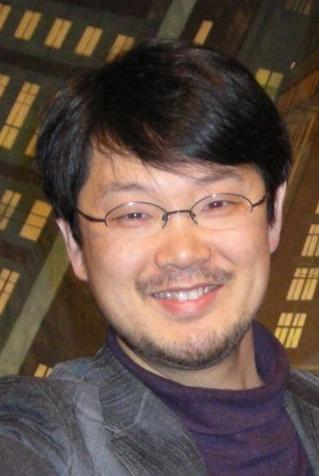
\includegraphics[width=70pt]{images/matz.jpg}
\end{center}

\begin{itemize}
	\item Ruby was created on February 24, 1993 by Yukihiro Matsumoto\\
			who wished to create a new language that balanced \emph{\textcolor{blue}{functional}} programming with \emph{\textcolor{blue}{imperative}} programming.
	\item ``I wanted a scripting language that was \emph{more powerful than Perl}, and \emph{more object-oriented than Python}.''
	\item Ruby 1.0 was released on December 25, 1996
	\item Current Ruby version is 1.9.2 (released on September 18, 2010)
\end{itemize}
\end{frame}

% Who use Ruby ?
\begin{frame}{Who use Ruby ? \footnote{http://www.ruby-lang.org/en/documentation/success-stories/} }
\begin{itemize}
	\item NASA Langley Research Center uses Ruby to conduct simulations
	\item Google SketchUp is a 3D modeling application that uses Ruby for its macro scripting API
	\item Ruby On Rails is one of the best and most innovative web application framework (GitHub, Twitter, Basecamp, Scribd, Geni, Redmine, Lighthouse, Urban Dictionary, White Pages, Next Sprocket, spitzer.caltech.edu (NASA), Go vs Go, $\ldots$)
	\item Ruby was used to write the central data collection portion of Level 3 Communications Unix Capacity and Planning system that gathers performance statistics from over 1700 Unix servers scattered around the globe
\end{itemize}
\end{frame}

% Interpreters
% TODO: add interpreters logos
\begin{frame}{Interpreters}
\begin{itemize}
	\item MRI: Matz's Ruby Interpreter: C
	\item JRuby: Java
	\item Rubinius: Ruby on top of LLVM with C++
	\item MacRuby: Objective-C, bridge with Cocoa
	\item IronRuby: Open Source implementation for .NET
\end{itemize}
\end{frame}

% Main Principles
\begin{frame}{Main Principles}
\begin{itemize}
	\item Beautiful and natural syntax, no useless () \{\} ; $\ldots$
	\item Everything is an Object: Number, Class, Method, Binding, nil $\ldots$
	\item Dynamic typing and Duck typing
	\item Succinct and flexible syntax
	\item Reflection and metaprogramming
	\item Functional programming with Blocks/closures
\end{itemize}
\end{frame}

% Syntax
\begin{frame}[fragile]{Syntax}
\begin{lstlisting}
array = [1, [2.0, 'c'], :d, (5..67)]
obj.method(*params) { block }
# or obj.m(*params) do block end

class MyClass
  def my_method(*args)
    body
    this_last_statement_is_the_returned_value
  end

  def clever_params(a, b = a *2, c = @ivar**2)
  end
end

you, (can, splat), *an = array
\end{lstlisting}
\end{frame}

% Simplicity
\begin{frame}[fragile]{Simplicity}
\begin{lstlisting}[xleftmargin=40pt]
vowels = %w[a e i o u]

alphabet = ('a'..'z').to_a

consonants = alphabet - vowels
\end{lstlisting}
\end{frame}

% Expressiveness
\begin{frame}[fragile]{Expressiveness}
\begin{lstlisting}[xleftmargin=30pt]
5.times { puts 'Hello Ruby' }

"This is Ruby".length # => 12

3.even? # => false

[1,2,3].include? 2 # => true

ary.shuffle! until ary.sorted? # Bogosort
\end{lstlisting}
\end{frame}

% Productivity
\begin{frame}[fragile]{Productivity}
\begin{lstlisting}
class Person
 # def name
 #   @name
 # end
 # def name= name
 #   @name = name
 # end
 # ...
 attr_accessor :name, :age
end

john = Person.new
john.name = 'John'
john.age = 25
# or
Person = Struct.new(:name, :age)
\end{lstlisting}
\end{frame}

% Flexibility
\begin{frame}[fragile]{Flexibility}
Core classes can be modified, even Fixnum\#+
\begin{lstlisting}[xleftmargin=40pt]
class Array
  def shuffle
    sort_by { rand }
  end
end

[1, 2, 3].shuffle # => [2, 3, 1], ...
\end{lstlisting}
\end{frame}

% Dynamism
\begin{frame}[fragile]{Dynamism}
\begin{lstlisting}[xleftmargin=-10pt]
Padawan = Class.new
class Jedi
  def train(padawan)
    def padawan.control_the_force
      puts "Now i'm ready to become a Jedi!"
    end
  end
end

Skywalker, Yoda = Padawan.new, Jedi.new
Skywalker.respond_to? :control_the_force # => false

Yoda.train Skywalker
Skywalker.respond_to? :control_the_force # => true
Skywalker.control_the_force
# => Now i'm ready to become a Jedi!
\end{lstlisting}
\end{frame}

% Conciseness
\begin{frame}[fragile]{Conciseness}
\begin{lstlisting}[xleftmargin=30pt]
require 'sinatra'

get '/' do
  'Hello, World!'
end

$ curl localhost:4567 # => Hello, World!
\end{lstlisting}
\end{frame}

% Beautiful API
\begin{frame}[fragile]{Beautiful API}
\begin{lstlisting}[xrightmargin=-10pt]
open('ruby-conf.rb') { |f| f.write 'New Orleans' }

# URI work too !
require 'open-uri'

puts open 'http://www.ruby-lang.org/en/', &:read
\end{lstlisting}
\end{frame}

% Simplify loops
\begin{frame}[fragile]{Simplify loops}
\begin{lstlisting}
def factorial n
  fact = 1
  for i in (1..n)
    fact *= i
  end
  return fact
end
factorial(5) # => 120

# becomes
class Integer
  def !
    (1..self).inject(1) { |fact, i| fact * i }
  end
end
5.! # => 120
# can even be: (1..self).inject(1, :*)
\end{lstlisting}
\end{frame}

% Chaining
\begin{frame}[fragile]{Chaining}
\begin{lstlisting}[xrightmargin=-10pt]
[450, 1000, 675].sort.take(2).map { |p| "$#{p}" }
# => ["$450", "$675"]

# Find the char with the most occurrences in a String
adn = "ATTGCCATATCC".chars.to_a
adn.uniq.sort.max_by { |c| adn.count(c) } # => "C"
\end{lstlisting}
\end{frame}

% Enumerators
\begin{frame}[fragile]{Enumerators}
\begin{lstlisting}
# has a gap after 4 and 7!
numbers = [1, 2, 3, 4, 6, 7, 9, 10]

gaps = []
numbers.each_cons(2) do |x, y|
  gaps << x unless y == x + 1
end
gaps #=> [4, 7]

# or

numbers.each_cons(2)
  .reject { |x,y| x + 1 == y }.map(&:first)
\end{lstlisting}
\end{frame}

% Caching
\begin{frame}[fragile]{Caching}
\begin{lstlisting}
# Caching is easy: we have the ||= operator
# which assign only if it is nil or false

def my_method
  @cache ||= some_extensive_computation
end
\end{lstlisting}
\end{frame}

% Closures
\begin{frame}[fragile]{Closures}
\begin{lstlisting}
def create_get_and_set closure_value
  return lambda { closure_value },
     lambda { |x| closure_value = x }
end
 
getter, setter = create_get_and_set
setter.call(42)
getter.call # => 42
\end{lstlisting}
\end{frame}

% Operators
\begin{frame}[fragile]{Operators}
Name it as it is, operators are just methods:
\begin{lstlisting}
1 + 2 == 1.+(2)

class Number
  # Same for + / % ** & ^ | << [] []= ~ < ...
  def * n
    @value * n
  end
end
\end{lstlisting}
\end{frame}

% Literals
\begin{frame}[fragile]{Literals}
Most useful objects are literals
\begin{lstlisting}[xleftmargin=20pt]
[1, 2_345_678, 0xfe, 0b101010]
3.14
"string"
/RegExp/
:symbol
%w[array of strings]
range = (1..15)
hash = {key: value}

<<HERE
heredoc
HERE
\end{lstlisting}
\end{frame}

% String interpolation
\begin{frame}[fragile]{String interpolation}
\begin{lstlisting}[xleftmargin=20pt]
"This is #{'*so* ' if $VERBOSE}useful !"

"There is real #{sleep 1}code"

"I love #{"nest#{'ing'}"}"

"It convert to #{String} by calling #to_s"
\end{lstlisting}
\end{frame}

% Rich stdlib
\begin{frame}[fragile]{Rich stdlib}
All core Classes have a lot of handy methods
\begin{lstlisting}
Array.instance_methods # => ..., pop, push, shift, unshift, take, drop, insert, replace, [], []=, rotate, ...
String.instance_methods # => bytes, capitalize, center, chars, chomp, chop, codepoints, downcase, lines, end_with?, (g)sub(!), encode ...
Enumerable.instance_methods # => count, grep, min, min_by, sort_by, each_with_index, map, each_cons, each_slice, zip, take, ...
\end{lstlisting}
\end{frame}

% Scripting
\begin{frame}[fragile]{Scripting}
\begin{lstlisting}[literate={`}{{$^{\backprime}$}}1]
# set_mtime_from_exiftime

#!/usr/bin/env ruby
require 'time'
Dir["**/*.{jpg,JPG}"].each do |f|
  times = `exiftime #{f}`
  .scan(/(?:\d+:\d+:\d+ ?){2}/)
  .map { |time| Time.new(*time.split(/\W/) }

  raise "Not same times: #{times}" unless times.all? { |time| time == times.first }
  File.utime(File.atime(f), times.first, f)
end
\end{lstlisting}
\end{frame}

% RSpec
\begin{frame}[fragile]{RSpec}
\begin{lstlisting}
describe BlogPost do
  subject { BlogPost.new 'foo', 'bar' }
  it { should be_invalid }
end

describe Array do
  its(:length) { should == 0 }
end

expect do
  foo.bar
end.to change { baz.quux }.by(1)

mock.should_receive(:method).once.with(args).and_return(answer)
\end{lstlisting}
\end{frame}

% A quote of Matz
\begin{frame}{A quote of Matz}
``[...] The computers don't care. We humans care about the effort we pay. Often people, especially computer engineers, focus on the machines. They think, ‘By doing this, the machine will run faster. By doing this, the machine will run more effectively. By doing this, the machine will something something something.’ They are focusing on machines. But in fact we need to focus on humans, on how humans care about doing programming or operating the application of the machines. We are the masters. They are the slaves.'' \footnote{http://www.artima.com/intv/ruby4.html}
\end{frame}

% Credits
\begin{frame}{Credits}
\begin{itemize}
	\item http://ruby-lang.org
	\item Wikipedia: Ruby, Yukihiro Matsumoto
	\item ruby-talk: ``The beauty of Ruby through examples''
	\item Pure RSpec: http://pure-rspec-scotruby.heroku.com
	\item RSpec: http://rspec.info
\end{itemize}
\end{frame}

\end{document}

% Any barrier that exists between the user and some part of the system will eventually be a barrier to creative expression.
% Any part of the system that cannot be changed or that is not sufficiently general is a likely source of impediment.
% If one part of the system works differently from all the rest, that part will require additional effort to control.
% Such an added burden may detract from the final result and will inhibit future endeavors in that area.


